\section{はじめに}
\subsection{人間の嗅覚}
\label{subsec:intro}
人間の食べる時に使う感覚は舌による味覚だけではなく,嗅覚,視覚,聴覚,触覚の五感すべて
によって刺激から感じる. 本研究では,その中でも味覚に注目して,味覚に関係性が深い嗅覚に
着目した.嗅覚は,食べ物の香りを感じる時にとても敏感に働く感覚である.食べる前に香りを
嗅ぐと,食欲を増大させる.他に,食事の良し悪しや好き嫌いを判断する時にも,必要となる感
覚である.その情報が味覚の感覚に影響を与え,感じ方を変化させるため「味」に大きな影響を
与えていると言われている.


\subsection{オルソネーザルアロマとレトロネーザルアロマ}
嗅覚には図\ref{kyukaku}で示したようにオルソネーザルと言われる鼻から入る香りとレトロネーザルと
言われる口から入り鼻から抜ける香りの2つがある.鼻をつまむと味がしなくなる現象や風邪な
ど鼻の不具合により味がしなくなる現象から嗅覚は味覚に影響があることが分かる.オルソネー
ザルの場合は,鼻から生じる単独の感覚であり,香りに特化した知覚である.一方,レトロネー
ザルは口内から入るため,味覚や感覚,触覚も加わることから複数の感覚が連動して新たな風味
が形成される.


\begin{figure}[t]
    \centering
    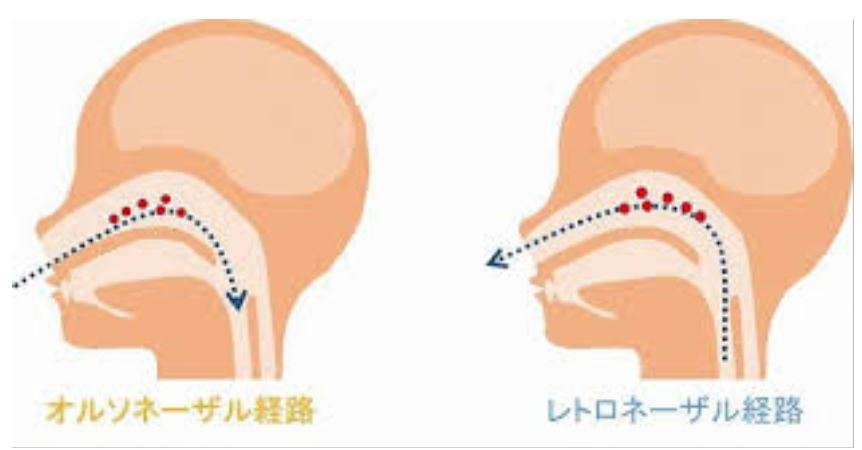
\includegraphics[width = 1.1\columnwidth]{kyukaku.JPG}
    \caption{オルソネーザルとレトロネーザル}
    \label{kyukaku}
  \end{figure}


\subsection{研究の目的}
レトロネーザルはオルソネーザルよりも複数の感覚から風味を感じやすいと考える.そのため
レトロネーザルを利用し,口の中から香りを与え嗅覚に刺激を与えることで風味を感じさせるこ
とが出来ると考えた.このように嗅覚刺激による風味,味覚への変化を検証する研究は存在する
が,食べられるものを使い香りを与えるものは少ない.チューブによって香りを嗅覚に与えるデ
バイスが多いため,食べれるものでの仕組みを作り出すことで口の中にチューブを入れるなどの
問題点を解決できるのではないかと考えた.


本稿では,口の中に香りを与える方法として,アガーで作成したゼリーの中に香りを閉
じこめたものを用意した.無味無臭の球体のゼリーの中に香りを閉じこめることで,口の中に香
りを与えることができると考えた.この香りによって人間が飲食するときにおいて感じる風味を
与えることができる.この仕組みにより風味にどのような差異があるか調査し,研究をしていく.